\makeatletter\@specialfalse\makeatother
\cxset{style13}
\chapter{Introduction}
\addtocimage{-12pt}{-20pt}{../images/tocblock-fish.jpg}


\epigraph{``Begin at the beginning,'' the king said
"and then go on till you come to the end, then stop."}{
---Lewis Carroll, Alice in Wonderland}

\begin{verbatim}
  \chapter{Drawing pictures and graphs}
\epigraph{Dear God\break If I have but one hour remaining to live, please allow me to spend this time
in a mathematics class so that it will seem to last forever.}{\textit{---A bored student's prayer}}


\begin{figure}%
  \centering
  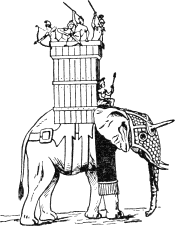
\includegraphics[width=0.3\linewidth]{./graphics/pic37.png}
  \caption{During the early days of typography fonts were designed to emulate the looks of calligraphic texts.}
  \label{fig:marginfig1}
\end{figure}

\section{Inserting figures}

In order to insert figures, the \pkgname{graphicx} package has to included in the preamble (before the |\begin{document}|-command) of your LaTeX-document:

\graybox{\texttt{\textbackslash usepackage\{graphicx\}}}

Originally only EPS-figures could be inserted with the \pkgname{graphic}package. This has now been developed into the  \pkgname{graphicx}, which allows almost any common format to be inserted. 

The simplest way of including a graphic looks like this:


\CMDI{\includegraphics}\marg{filename}


If the image is not located in the same folder as the tex-file, you will have to specify the path relative to the tex-file.

\graybox{\texttt{\textbackslash includegraphics\{./images/filename\}}}


\subsection{Scaling and resizing images}

If you want the image to appear in a different size, you can specifiy the size as a parameter of the |\includegraphics|-command::


\graybox{\texttt{\textbackslash includegraphics[width=3.9cm]\{filename\}}}


This will scale the image to the width of 3.9 centimeters. 

Use |\textwidth| command if you don't want to specify an absolute size but rather want the actual size to depend on the text width of the page. You can use any of the normal \tex units such as \texttt{em, pt, cm, in}:
\graybox{\texttt{\textbackslash includegraphics[width=0.5\textbackslash textwidth]\{filename\}}}
\noindent will scale the image to half of the text width. The images in the
figure below were produced by two |includegraphics| commands. You can have as many as you like and the \tex engine will treat them the same way as text. If you a leave a space between the commands, they will be positioned vertically as they are treated as paragraphs.

\medskip
\begingroup

\centering
\includegraphics[width=0.3\textwidth]{./graphics/amato.jpg}
\includegraphics[width=0.3\textwidth]{./graphics/amato.jpg}
\includegraphics[width=0.3\textwidth]{./graphics/amato.jpg}

\endgroup


The three photos were centered using the |\centering| command, within a group.


\begin{teX}
\begingroup

\centering
\includegraphics[width=0.3\textwidth]{./graphics/amato.jpg}
\includegraphics[width=0.3\textwidth]{./graphics/amato.jpg}
\includegraphics[width=0.3\textwidth]{./graphics/amato.jpg}
\endgroup
\end{teX}

The |\begingroup..\endgroup| is necessary to limit the effect of centering to
the group only, otherwise \tex would center everything from this point onwards.

\subsection{Controlling the aspect ratio}

You can control the picture aspect ratio by using the command:

\CMDI{\includegraphics}[keepaspectratio,width=3cm, height=3cm]]\{filename\}


If set to true then specifying 
both |width| and |height| (or |totalheight|) does not distort the figure but 
scales such that neither of the specified dimensions is exceeded.






\medskip
\begingroup

\centering
\includegraphics[width=0.3\textwidth, height=5cm]{./images/amato.jpg}
\includegraphics[keepaspectratio=true,width=4cm, height=5cm]{./images/amato.jpg}
\includegraphics[width=3cm]{./images/amato.jpg}

\endgroup


This can be very useful if you have images shown side by side with different
aspect ratios. 


\subsection{Paths and file types}

For larger projects you will probably find it more convenient to have 
images in different folders. You can specify default paths using:


\CMDI{\graphicspath}\marg{dir-list}

This optional declaration may be used to specify a list of directories in which to
search for graphics files. The format is the same as for the \latexe primitive
|\input@path|. A list of directories, each in a \{\} group (even if there is only one
in the list). For example:


\graybox{\texttt{\textbackslash graphicspath\{\{eps/\}\{tiff/\}\}}}


The default image formats can be declared using:

\CMDI{\DeclareGraphicsExtensions}\marg{png,jpg}

This specifies the behaviour of the system when no file extension is specified in 
the argument to |\includegraphics|. \texttt{\{ext-list\}} should be a comma separated 
list of file extensions. (White space is ignored between the entries.) A file name
is produced by appending one extension from the list. If a file is found, the
system acts as if that extension had been specified. If not, the next extension
in \texttt{ext-list} is tried.



\subsection{The figure environment}

You use the figure-environment to let your image appear in a "floating" environment, that is \latex will place it at the right position of a page and even on the next page:

\begin{teX}
\begin{figure}
  \includegraphics{filename.eps}
  \caption{title of your figure}
  \label{labelname}
\end{figure}
\end{teX}

Here |\caption{...}| defines the title of the figure which will appear beneath the figure. |\label{..}| defines the label which can be used inside the document in order to insert references to the figure:

The figure

|\ref{labelname} on page \pageref{labelname} ..|

The|\label-command| inside the |\figure|-envirnonment hast to appear just after the|\caption|-command.
placing figures

If figures reside inside a |\figure|-environment, this will cause LaTeX to choose the actual location of the figure inside the document. There are different parameters for the placement strategy:

\begin{description}
\item[h (here)] Try to place the figure just where the command is located.

\item [t (top)] Try to place the figure at the top of the page.

\item[b (bottom)] Try to place the figure at the bottom of the page.

\item [p (float page)] Try to place the figure on a page which contains only floating elements.
\end{description}

The order of these parameters doesn't matter since placement is always tried in the order \textbf{h, t, b, p,} if these parameters are present:

If no parameter is present, the default order is  \texttt{[tbp]}.


The command for a figure-environment might for example look like this:

\begin{teX}
\begin{figure}[htbp]
...
\end{figure}
\end{teX}



\subsection{Table of figures}
\index{figures!Table of figures}
A table of figures is inserted (where you place the command) using the command


\begin{teX}
   \listoffigures
\end{teX}

The caption given in the \cmd{caption} command is also used in the list of figures. 
If you want to use different captions, you may add a parameter to the |\caption| command:
|\caption[caption for listoffigures]{caption inside the document}|


\subsection{Figures with a border}

Although drawing frames around tables should be discouraged, if you find the need
to draw them there are  two possible ways to achieve it: either only the figure itself is bordered or there is a border around the figure and its caption. You place a border around the figure using the \cmd{\fbox} command or the \cmd{\framebox}.

\emphasis{fbox,minipage}
\begin{teX}
\begin{figure}[htbp]
  \centering
  \fbox{
    \includegraphics{filename}
  }
  \caption{caption}
  \label{Labelname}
\end{figure}
\end{teX}

Placing a border around the figure and its title is a little more tricky: You need to place the figure and the title in a |\minipage| environment which is bordered again with the |\fbox| command:

\begin{teX}
\begin{figure}[htbp]
  \centering
  \fbox{
    \begin{minipage}{13 cm}
      \includegraphics{filename}
      \caption{caption}
      \label{labelname}
    \end{minipage}
  }
\end{figure}
\end{teX}

This will produce the image shown below,

\begin{center}
\begin{figure}[htbp]
  \centering
  \fbox{
    \begin{minipage}{0.25\linewidth}
      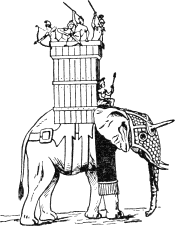
\includegraphics[width=0.9\linewidth]{./graphics/pic37.png}
      \caption{The boxed fighting elephant}
      \label{labelname}
    \end{minipage}
  }
\end{figure}
\end{center}


Unfortunately the width of the border cannot be determined automatically. It has to be specified as a parameter of the |\minipage| environment. However, you may be bale to develop a macro to do this - based on the ImageSize routines we developed in section.


\section{Side by side figures}

You might want to place to figures side by side but to use only one caption. This is achieved by placing both figures in its own |\minipage| which reside in the same |\figure|.

if only one |\caption| command is used, both figures will have a common title:

\medskip
\begin{verbatim}
\begin{figure}[htbp]
  \centering
  \begin{minipage}[b]{5 cm}
    \includegraphics{filename 1}  
  \end{minipage}
  \begin{minipage}[b]{5 cm}
    \includegraphics{filename 2}  
  \end{minipage}
  \caption{common caption}
  \label{Labelname}
\end{figure}
\end{verbatim}
\medskip

The first parameter of the |\minipage| environment determines how both graphics are aligned to each other. b (bottom) aligns the bottom borders of the figures, \textbf{t} (top) aligns the top borders and \textbf{c} aligns the centers.

If you want distinct titles for the two figures you will only have to supply a |\caption| command for both |\minipage|environments:

\begin{teX}
\begin{figure}[htbp]
  \centering
  \begin{minipage}[b]{5 cm}
    \includegraphics{filename 1} 
    \caption{caption 1}
    \label{labelname 1}
  \end{minipage}
  \begin{minipage}[b]{5 cm}
    \includegraphics{filename 2}  
    \caption{caption 2}
    \label{labelname 2}
  \end{minipage}
\end{figure}
\end{teX}


If you want to have subfigures with distinct caption, you use the |\subfig| package:


You can put as many figures as you like on a page, but a word of warning, you may need to make some manual adjustments before you get it right. The package provides support for the manipulation and reference of small or ‘sub’ floats within a single floating (e.g., figure or table) environment1 It is convenient to use this
package when your sub-floats are to be separately captioned, referenced, or when such
sub-captions are to be included on a List-of-Floats page.

The package is a replacement for the subfigure package, from which it was derived.
However, the new subfig package is not completely backward compatible.
Therefore, a new name was called for. The newer package is smaller and easier to use
than the older package, however, it now uses the following additional packages, 
caption (required), 
everysel (optional), 
keyval (required), 
ragged2e (optional).

It will work without the ragged2e and everysel packages if you do not use the following
justification options: ‘Center’, ‘RaggedRight’ and ‘RaggedLeft’. The other justification
options ‘center’, ‘raggedright’ and ‘raggedleft’ will work without the above two packages. If the ragged2e package is present, than the caption package will load it and it
will, in turn, load the everysel package. This happens whether or not you will be using
the justification options that require it. If it cannot find the ragged2e package, than the
caption package will print a message that ‘RaggedRight’, etc. will not be available.



 A low bottle-shaped vase, of yellowish ware, with flaring rim and somewhat flattened body. Height, 5 inches; width 5 inches. \ref{fig:one}

A well-made bottle shaped vase, with low neck and globular body, somewhat conical above. Color dark brownish. 7½ inches in height. Shown in \ref{fig:two}


\begin{figure}
  \centering
  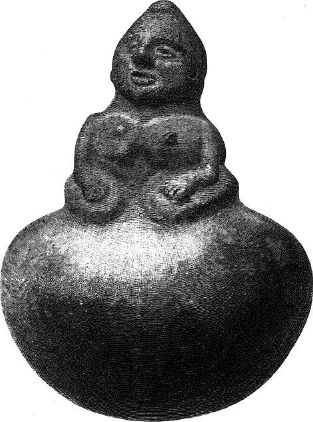
\includegraphics[width=0.7\linewidth]{./graphics/fig175.jpg}
   \centerline{From the tomb of a Pull\= arius.}
  \label{fig:marginfig1}
\end{figure}

The above figure is an effigy vase of the dark ware. The body is globular. A kneeling human figure forms the neck. The mouth of the vessel occurs at the back of the head—a rule in this class of vessels. Is is finely made and symmetrical. 9¾ inches high and 7 inches in diameter. being larger than the above two it is preferable to scale it to give the reader an indication. Based on the figure width, you may also need to adjust the distance between the figures to ensure that the whitespace is just about right. For screen reading this can be increased and for printed works you may wish to make it less.







\section{The wrapfig package}


\captionsetup[wrapfigure]{margin=10pt,font=small,labelfont=bf, name=Fig.} % [wrapfigure]{name=Fig.}


Donald Arseneau has created the \pkg{wrapfig} package to allow people to place figures or
tables at the side of a page and wrap text around them. The package provides the
environments wrapfigure and wraptable. Both environments have two required and
two optional arguments. You can see an example taht uses the package to wrap a picture into such a paragraph of text.

\begin{figure}[82pt]
   \includegraphics[width=\linewidth]{./graphics/cyprus.jpg} 
   \caption{\small Cyprian limestone group of Phoenician dancers, about 6½ in. high. There is a somewhat similar group, also from Cyprus, in the British Museum. The dress, a hooded cowl, appears to be of great antiquity.}
\end{figure}

\begin{wrapfigure}[20]{l}{3.8cm}
\centering\small
\includegraphics[width=\linewidth]{./graphics/egyptdance.jpg}  
\caption{\small The hieroglyphics describe the dance.}
\end{wrapfigure}
Amongst the earliest representations that are comprehensible, we have certain Egyptian paintings, and some of these exhibit postures that evidently had even then a settled meaning, and were a phrase in the sentences of the art. Not only were they settled at such an early period (B.C. 3000, fig. 1) but they appear to have been accepted and handed down to succeeding generations (fig. 2), and what is remarkable in some countries, even to our own times. The accompanying illustrations from Egypt and Greece exhibit what was evidently a traditional attitude. The hand-in-hand dance is another of these.

The earliest accompaniments to dancing appear to have been the clapping of hands, the pipes,[1] the guitar, the tambourine, the castanets, the cymbals, the tambour, and sometimes in the street, the drum.

The following account of Egyptian dancing is from Sir Gardiner Wilkinson's "Ancient Egypt"[2]:—
\begin{figure}
   \includegraphics[width=0.3\linewidth]{./graphics/lotus.jpg} 
   \caption{\small Cyprian limestone group of Phoenician dancers, about 6½ in. high. There is a somewhat similar group, also from Cyprus, in the British Museum. The dress, a hooded cowl, appears to be of great antiquity.}
\end{figure}
"The dance consisted mostly of a succession of figures, in which the performers endeavoured to exhibit a great variety of gesture. Men and women danced at the same time, or in separate parties, but the latter were generally preferred for their superior grace and elegance. Some danced to slow airs, adapted to the style of their movement; the attitudes they assumed frequently partook of a grace not unworthy of the Greeks; and some credit is due to the skill of the artist who represented the subject, which excites additional interest from its being in one of the oldest tombs of Thebes (B.C. 1450, Amenophis II.). Others preferred a lively step, regulated by an appropriate tune; and men sometimes danced with great spirit, bounding from the ground, more in the manner of Europeans than of Eastern people. On these occasions the music was not always composed of many instruments, and here we find only the cylindrical maces and a woman snapping her fingers in the time, in lieu of cymbals or castanets.

\begin{figure}
   \includegraphics[width=0.3\linewidth]{./graphics/patera.jpg} 
   \caption{\small Cyprian limestone group of Phoenician dancers, about 6½ in. high. There is a somewhat similar group, also from Cyprus, in the British Museum. The dress, a hooded cowl, appears to be of great antiquity.}
\end{figure}

"Graceful attitudes and gesticulations were the general style of their dance, but, as in all other countries, the taste of the performance varied according to the rank of the person by whom they were employed, or their own skill, and the dance at the house of a priest differed from that among the uncouth peasantry, etc.

"It was not customary for the upper orders of Egyptians to indulge in this amusement, either in public or private assemblies, and none appear to have practised it but the lower ranks of society, and those who gained their livelihood by attending festive meetings.

"Many of these postures resembled those of the modern ballet, and the pirouette delighted an Egyptian party 3,500 years ago.
\medskip

The wrapped figure is positioned using the \texttt{wrapfigure} environment, as shown below:

\begin{teX}
\begin{wrapfigure}[nlines]{placement}[overhang ]{width }
   \includegraphics[width=3.8cm]{./graphics/egyptdance} 
   \caption{\small The hieroglyphics describe the dance.}
\end{wrapfigure}
\end{teX}

The parameter |nlines|  is the number of narrow lines, and placement is one of r, l, i, o, R, L, I, or
O for right, le, inside, and outside, respectively. The uppercase placement specifiers
differ from their lowercase counterparts in that they force \latex to put the float \emph{here},
whereas the lowercase placement specifiers just give a hint to \latex to place them
\texttt{here}. The \texttt{width} argument is the width of the figure or table that appears in the body
of the environment. Finally, \texttt{overhang} tells LATEX how much the figure should hang out
into the margin of the page. Here is how one may create dangerous paragraphs bends!

The |wrapfig| package is compatible with the |caption| package. You can set the caption parameters using:---

\begin{teX}
\captionsetup[wrapfigure]{<options>}
\end{teX}

If you are probably wondering how |wrapfig| achieves this, you should read the class file. It basically uses |everypar|, and hence the limitations with |\par|. Here is an extract from the class.

\begin{teX}

% Subvert \everypar to float fig and do wrapping.  
% Also for non-float.
\def\WF@startfloating{%
 \WF@everypar\expandafter{\the\everypar}\let\everypar\WF@everypar
 \WF@@everypar{\ifvoid\WF@box\else\WF@floathand\fi \the\everypar
 \WF@wraphand
}}
\end{teX}

Moving now to a more scientific example that the previous ones, we will place two figures
one on top of each other and give them individual, sub-captions as shown in \ref{fig:honey}.
 
\captionsetup[figure]{margin=10pt,font=small,labelfont=bf,format=hang}%

\begin{figure}[htbp]
\centering
  \begin{subfigure}[b]{0.5\textwidth}
  \includegraphics[width=\linewidth]{./graphics/honey.png}
  \caption{Taylor instability in the surface of the honey in an inverted honey jar.}\label{fig:honey}
    \hspace{1cm}
  \end{subfigure}

  \begin{subfigure}[b]{0.9\textwidth}
     \centering
     \includegraphics[width=9cm]{./graphics/honeydrops.png}
     \caption{Taylor instability in the interface of the water condensing on the underside of a small water pipe.}
  \end{subfigure}  
  \caption{Two examples of Taylor instabilities that are commonly found.}%
    \label{fig:Athird}%
\end{figure}

The figures are from A Heat Transfer Textbook, by J.H.Lienhard, which incidentally was typeset using
\tex . It is a McGrawHill publication. 

\begin{teX}
\begin{figure}[htbp]
    \captionsetup[figure]{margin=10pt}%
    \subfloat[Taylor instability...]
     {{\includegraphics[width=8cm]{./graphics/honey}}}
    \hspace{1cm}
     \subfloat[Taylor instability in the...]%
      {\includegraphics[width=9cm]{./graphics/honeydrops}}  
     \\[-10pt]
   \caption{Taylor instability in...}%
    \label{fig:Afirst}%
    \caption{Two examples of... }%
    \label{fig:honey}%
\end{figure}
\end{teX}


The text can have more than one paragraph. It is also possible to include figures
generated by |TikZ/pgf|, as shown in the next example, drawn from real code
in the book.


\begin{wrapfigure}[14]{l}{3.0cm}
\pgfplotsset{width=5.0cm,compat=1.3}
\begin{tikzpicture}
\begin{axis}[minor y tick num=4, 
minor x tick num=4, 
xmin=0,xmax=300,
ymin=0,ymax=60,
xlabel=\textsf{liquidus ($l/s$)},
ylabel=\textsf{capitis ($m$)}, 
ytick={0,15,30,45,60,75},
xtick={0,100,200,300}
]
\addplot[color=blue,mark=x, smooth] coordinates {
(0,44)
(50,43)
(100,42)
(150,40)
(200,33)
(220,29)
};

\end{axis}
\end{tikzpicture}
\caption{Pump headum and flowm}
\end{wrapfigure}


\providecommand\addcredit[1]{%
 \vspace*{-6.5pt}
 \scriptsize%
 \flushright%
 \textit{Credit: #1}%
}
\newpage
\pagestyle{empty}
\thispagestyle{empty}
\begin{figure}[htp]
\centering

\captionsetup{name=Photo., labelsep=period}%
   \begin{minipage}[t]{0.48\textwidth}
      \includegraphics[width=\textwidth]{./graphics/movingup.jpg}%
      \addcredit{U.S. DoD.}%
     \caption{The effects of the credit going past the edge of the figure. This can be corrected by adding a minipage to hold both commands. }
\end{minipage}\hfill\hfill
\begin{minipage}[t]{0.48\textwidth}
      \includegraphics[width=\textwidth]{./graphics/survivors.jpg}%
      \addcredit{U.S. DoD.}%
    {\footnotesize Marines awaiting resting before moving on to Japan. }
\end{minipage}

% \begin{minipage}[t]{0.48\textwidth}
%      \includegraphics[width=\textwidth]{./graphics/img009.jpg}%
%      \addcredit{U.S. DoD.}%
%     \caption{Engineer Construction Troops in Liberia, July 1942.}
%\end{minipage}\hfill\hfill
%\begin{minipage}[t]{0.48\textwidth}
%      \includegraphics[width=\textwidth]{./graphics/survivors.jpg}%
%      \addcredit{U.S. DoD.}%
%     \caption{The effects of the credit going past the edge of the figure. This can be corrected by adding a minipage to hold both commands. }
%\end{minipage}
% \begin{minipage}[t]{0.48\textwidth}
%      \includegraphics[width=\textwidth]{./graphics/img126.jpg}%
%      \addcredit{U.S. DoD.}%
%     \caption{Marine Reinforcements.
%A light machine gun squad of 3d Battalion, 1st Marines, arrives during the battle for ``Boulder City.'' }
%\end{minipage}\hfill\hfill
%\begin{minipage}[t]{0.48\textwidth}
%      \includegraphics[width=\textwidth]{./graphics/img124.jpg}%
%      \addcredit{U.S. DoD.}%
%     \caption{Brothers Under the Skin, inductees at Fort Sam Houston, Texas, 1953. }
%\end{minipage}
\end{figure}
\newpage


Armed with all these packages you can help the Gutenburg organization to transcribe
some of the old books that they have online. 

\clearpage








  \chapter{WRAPPED ILLUSTRATIONS}
\parindent2em
\let\onepar\lorem

If you are planning to have a more traditional book design wrapped figures are essential. Traditional typographers used
all sorts of styles to achieve this is to use
The best way to achieve it is to use Donald Arseneau's wrafig package.

\begin{wrapfigure}{l}{3.2cm}
    \includegraphics[width=3cm]{amato}
    \caption{\footnotesize Wrapped figures}
\end{wrapfigure}

Get prepared to do a lot of manual adjustments, see your figures disappear on page refreshes and reruns. After a while though you get the hang of it and by minor adjustments you can really achieve great results. The manual uses \verb+everypar+ to insert commands for the shaping of the paragraphs that \emph{follow} the wrapped figure.

Wrapfig.sty provides the environments \pkg{wrapfigure} and \pkg{wraptable} for typesetting a
narrow float at the edge of the text, and making the text wrap around it. The wrapfigure
and wraptable environments interact properly with the \verb+\caption+ command to produce
proper numbering, but they are not regular floats like figure and table, so (beware!)
they may be printed out of sequence with the regular floats. The environment  provides one of those monster commands that stresses one's memory as itprovides for four parameters. 
The four param
for \verb+\begin{wrapfigure}+, two optional and two required, plus the text of the figure, with a caption perhaps.

\begin{macro}{wrapfigure}
\end{macro}

|\begin{wrapfigure}[12]{r}[34pt]{5cm}\meta{figure}\end{wrapfigure}|

  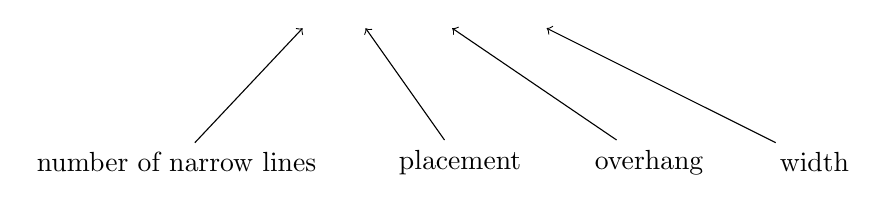
\begin{tikzpicture}[xshift=-15pt]
    \node (number) at (0mm, 0mm) {\oarg{number of narrow lines}};
    \node (placement) at (36mm, 0mm) {\marg{placement}};
    \node (overhang) at (60mm, 0mm) {\oarg{overhang}};
    \node (width) at (81mm, 0mm) {\marg{width}};
    \begin{scope}[->]
    \draw (number) -- (16mm, 17mm);
    \draw (placement) -- (24mm, 17mm);
    \draw (overhang) -- (35mm, 17mm);
    \draw (width) -- (47mm, 17mm);
    \end{scope}
  \end{tikzpicture}


First we will look at placing the figure without the use of optional commands.


\begin{verbatim}
\begin{wrapfigure}{r}{.4\textwidth}
    \includegraphics[width=.4\textwidth]{./path/file}
    \caption{\footnotesize Wrapped figures}
\end{wrapfigure}
\end{verbatim}

From the four parameters the first one indicates if the figure is to be typeset left or right.

\begin{verbatim}
\begin{wrapfigure}{l}{\imagewidth}
    \includegraphics[width=\imagewidth



]{./graphics/parasol-01}
    \caption{\footnotesize Wrapped figures}
\end{wrapfigure}
\end{verbatim}


\begin{wrapfigure}[16]{I}[0.1pt]{85pt}
    \vskip-10.5pt plus 2pt minus 2pt\relax
    \includegraphics[width=83pt]{parasol-01}
    \caption{\scriptsize Wrapped figures, parameters set at \texttt\{l\}\{90pt\}.}
\end{wrapfigure}

Changing the parameters to suit we now have the illustration floating to the left. Allowing for the figure to be approximately two point  wider than the actual graphic, will leave a bit more margin. If the figure is end low in the page you need to be careful, that it does not disappear, as you will not get any warning.

The first parameter we are going to use an optional parameter is the one that determines the number of narrow lines. The format is \verb+[narrowlines]{l}{90pt}+. Think of this parameter as a fine tuning parameter and do not touch it until after your final draft is ready. If you see indented lines at the beginning of the page that follows the wrapped figure, reduce the number of lines, until you get satisfactory results.

The second optional parameter, comes after the \texttt{\{r\}[overhang]} parameter.

The second optional parameter (\#3) tells how much the figure should hang out into
the margin. The default overhang is given by the length \verb+\wrapoverhang+, which is 0pt
normally but can be changed using |\setlength|. For example, to have all wrapfigures
use the space reserved for marginal notes,

\begin{verbatim}
\setlength{\wrapoverhang}{\marginparwidth}
\addtolength{\wrapoverhang}{\marginparsep}
\end{verbatim}

Again not recommended. The best approach is to specify the figures with O or I, let them float and if the results are
not very good then make manual adjustments. Get prepared to spend at least 5-10 minutes fiddling with the final result.

When you do specify the overhang explicitly for a particular figure, you can use a
special unit called \string\width meaning the width of the figure. For example, [0.5\string\width]
makes the center of the figure sit on the edge of the text, and [\string\width] puts the figure
entirely in the margin (and the adjacent text is indented by just \string\columnsep). This
\texttt{\string\width} is the actual width of the wrapfigure, which may be greater than the declared
width.

\begin{figure}[tb]
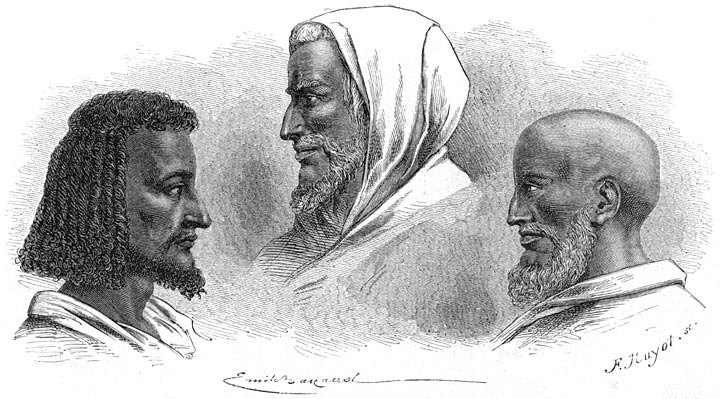
\includegraphics[width=\textwidth]{chiefs}
\caption{Chiefs of Kelau or Kelaou.}
\label{fig:chiefs}
\end{figure}

\begin{figure}[p]
\centering

\includegraphics[width=0.8\textwidth,height=0.9\textheight, keepaspectratio]{parasol-01}
\caption{Chiefs of Kelau or Kelaou.}
\label{fig:parasol-01}
\end{figure}

\section{Balancing the illustrations}

Illustrations come in various sizes, but in general they need to flow with the text. Place figures on top of the page and figures that would dominate the text on their own page. For example Figure~\ref{fig:chiefs} was allowed to float to the top of a page whereas Figure~\ref{fig:parasol-01} was placed on its own page, as I thought it will overwhelm the text if shown in a large size. However the same figure seems perfectly alright as a wrapped figure.

\begin{texexample}{}{}
\begin{wrapfigure}{I}{0pt}
    \includegraphics[width=75pt]{parasol-01}
 \end{wrapfigure}
\lipsum[1-2]
\begin{wrapfigure}{l}{0pt}
    \includegraphics[width=75pt]{parasol-01}
 \end{wrapfigure}
\lipsum[1-2]
\end{texexample}



\begin{texexample}{}{}
\begin{wrapfigure}{l}{0pt}
    \includegraphics[width=70pt]{parasol-01}
    \includegraphics[width=70pt]{parasol-01}
 \end{wrapfigure}

\lipsum[1-3]\lorem
\end{texexample}




\begin{texexample}{}{}
\begin{wrapfigure}[13]{L}{0pt}
    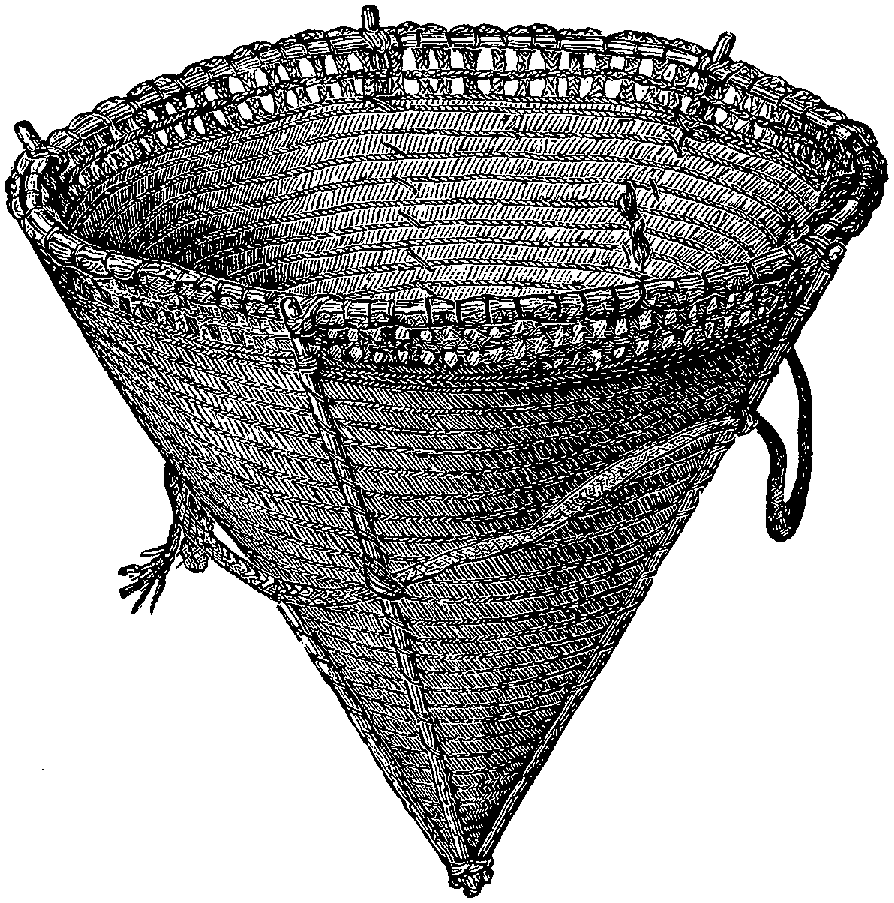
\includegraphics[width=100pt]{conicalbasket}
\end{wrapfigure}

\onepar\onepar\onepar

\end{texexample}




  \makeatletter
\newcommand\QEDit{\hspace{6pt}\textit{Q.~E.~D.}\quad}
\newcommand\QEFit{\hspace{6pt}\textit{Q.~E.~F.}\quad}
\newcommand\QEIit{\hspace{6pt}\textit{Q.~E.~I.}\quad}
\newcommand\QEDup{\hspace{6pt}Q.~E.~D.\quad}
\newcommand\QEFup{\hspace{6pt}Q.~E.~F.\quad}
\newcommand\QEIup{\hspace{6pt}Q.~E.~I.\quad}
\newcommand\QEOup{\hspace{6pt}Q.~E.~O.\quad}
\newcounter{wrapwidth}
\newcount \Zw
\newcount \Zh


\newcommand\pngright[4]{%
    \Zw=#2 \divide \Zw by 10
    \Zh=#3 \divide \Zh by 120  \advance\Zh by 1
    \setcounter{wrapwidth}{\Zw}
\begin{wrapfigure}[\Zh]{r}{\value{wrapwidth}pt}%
\begin{center}
\vspace{#4pt}%
\includegraphics*[width=\Zw pt]{images/#1}%
\end{center}
\end{wrapfigure}}

\newcommand\propnopage[1]{
\begin{center}{\large #1}\end{center}}

\parindent1em

\cxset{toc image=\@empty}
\chapter{PERICULA}

\noindent\textsc{Case Study: } We will now typeset a section, from Isaac Newton's \textit{Philosophi\ae\  Naturalis Principia Mathematica}. The typeset example is shown below.

\bottomline
\bgroup
\small

\cxset{section align=center,
         section numbering=none}

\section{{SECT}$\cdot$ VIII$\cdot$}

\begin{center}{\textit{De Motu per Fluida propagato.}}\end{center}

\makeatletter
%\propnopage{Prop.\ XLI\@. Theor.\ XXXI.}
\meaning\@
\makeatother

\textit{Pressio non propagatur per Fluidum secundum lineas rectas, nisi
ubi particul{\ae} Fluidi in directum jacent.}

Si jaceant particul{\ae} $a$, $b$, $c$, $d$, $e$ in linea recta, potest quidem
pressio directe

\begin{wrapfigure}[8]{O}[1pt]{0.3\textwidth}
  \vspace{-17pt}
  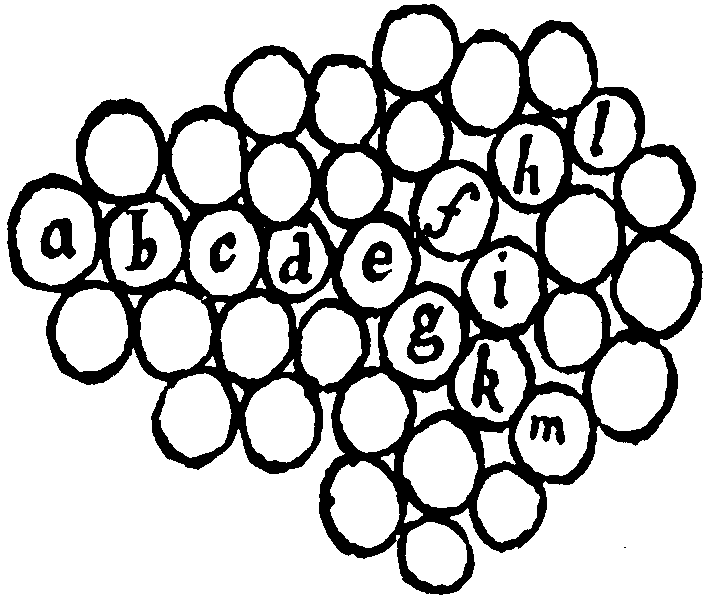
\includegraphics[width=0.27\textwidth]{images/362.png}
\end{wrapfigure}

\noindent propagari  ab $a$ ad $e$; at
particula $e$ urgebit particulas oblique positas
$f$ \& $g$ oblique, \& particul{\ae} ill{\ae} $f$ \& $g$
non sustinebunt pressionem illatam, nisi fulciantur
a particulis ulterioribus $h$ \& $k$;
quatenus autem fulciuntur, premunt particulas
fulcientes; \& h{\ae} non sustinebunt pressionem nisi fulciantur
ab ulterioribus $l$ \& $m$ easque premant, \& sic deinceps in infinitum.
Pressio igitur, quam primum propagatur ad particulas
qu{\ae} non in directum jacent, divaricare incipiet \& oblique propagabitur
in infinitum; \& postquam incipit oblique propagari, si
inciderit in particulas ulteriores, qu{\ae} non in directum jacent, iterum
divaricabit; idque toties, quoties in particulas non accurate
in directum jacentes inciderit. \QEDit

\topline

\vspace*{-\baselineskip}
\captionof{figure}{Example of a typeset page from Principi\ae.}
\egroup
\smallskip
Figure~\ref{fig:principia}, shows a scan of the actual page. We will not reproduce, the fonts and the page geometry exactly, but rather we will attempt to extract and reproduce the typographical rules employed in the printing of the \textit{Principi\ae}.

We begin by typesetting the section number and its heading. The use of roman numbers creates better harmony between the text and the heading

\begin{teX}
\sectpage{VIII$\middot$}
\begin{center}{\textit{De Motu per Fluida propagato.}}\end{center}
\end{teX}
The proposition and theorem line, has its own command
\begin{teX}
\makeatletter
\propnopage{Prop.\ XLI. Theor.\ XXXI.}
\makeatother
\end{teX}

\propnopage{\color{gray}Prop.\ XLI\@. Theor.\ XXXI.}
\vspace*{-37pt}
\propnopage{Prop. XLI. Theor. XXXI.}


Notice the small differences in the spacing with the commands as shown and with the black text, without them. The rest is based on normal \LaTeX\ commands.

\textit{Pressio non propagatur \ldots particul{\ae}\ldots}

\pngright{362.png}{709}{603}{-24}

Si jaceant particul{\ae} $a$, $b$, $c$, $d$,
$e$ in linea recta, potest quidem
pressio directe propagari ab $a$ ad $e$; at


Remember that it is important to start a new paragraph after the 
|pngright| command. The |wrapfig| package works by using |everypar| to insert the hanging indentation.

\begin{figure}[p]
\centering
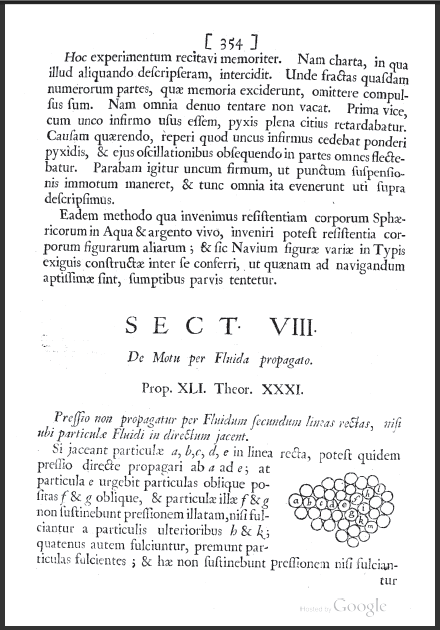
\includegraphics[scale=1]{./images/page354.png}
\caption{Page 354 from Isaac Newton's \textit{Philosophi\ae\  Naturalis Principia Mathematica}. Image was obtained from Google's copy, available at Google Books.}
\label{fig:principia}
\end{figure}
\makeatother

  \chapter{Subfigures}

So far we have been using the |caption| package to add captions to multiple figures, that are numbered individually, but how about if you want to have only one caption and number the subfigures alphabetically. If you want to have |subfigures| with distinct caption, you use the |subfig| package \citep{subfigure}. A newer package \ctan{subcaption} is also now available with the |caption| suite and we will discuss this also. The two packages are incompatible and the recommendation is to use the |subcaption| package. In the |phd| class we load the |caption| package which also loads the |subcaption| package. The latter is to be preferred as it integrates better both with captions as well as the |hyperref| package.

\begin{figure}[h]
\centering
\begin{minipage}[b]{.3\linewidth}
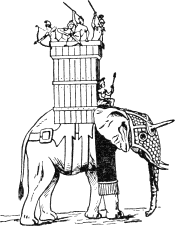
\includegraphics[width=4cm]{./graphics/pic37.png}\hspace{1em}
\subcaption{First fighting elephant}\label{fig:1a}
\end{minipage}\hspace{1em}
\begin{minipage}[b]{.3\linewidth}
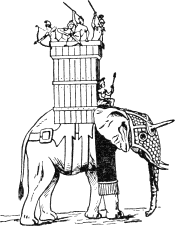
\includegraphics[width=4cm]{./graphics/pic37.png}\hspace{1em}
\subcaption{Second fighting  elephant}\label{fig:1b}
\end{minipage}\hspace{1em}
\begin{minipage}[b]{.3\linewidth}
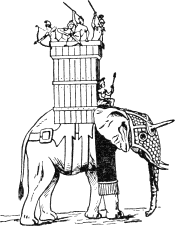
\includegraphics[width=4cm]{./graphics/pic37.png}\hspace{1em}
\subcaption{Third fighting elephant}\label{fig:1c}
\end{minipage}
\caption{Three fighting elephants example}
\end{figure}

You can put as many figures as you like on a page, but a word of warning, you may need to make some manual adjustments before you get it right. The package provides support for the manipulation and reference of small or \enquote{sub} floats within a single floating (e.g., figure or table) environment It is convenient to use this
package when your sub-floats are to be separately captioned, referenced, or when such
sub-captions are to be included on a List of Floats page.

The package is a replacement for the |subfigure| package, from which it was derived.
However, the new |subfig| package is not completely backward compatible.
Therefore, a new name was called for. The newer package is smaller and easier to use
than the older package, however, it now uses the following additional packages,  |caption| (required),  |everysel| (optional),
keyval (required),  |ragged2e| (optional). All these packages are included with the |phd| auto package manager.

It will work without the |ragged2e| and |everysel| packages if you do not use the following
justification options: \enquote{Center}, \enquote{RaggedRight} and \enquote{RaggedLeft}. The other justification
options \enquote{center}, \enquote{raggedright} and \enquote{raggedleft} will work without the above two packages. If the ragged2e package is present, than the caption package will load it and it
will, in turn, load the everysel package. This happens whether or not you will be using
the justification options that require it. If it cannot find the ragged2e package, than the
caption package will print a message that \enquote{RaggedRight}, etc. will not be available.

\section{Subcaption environments}

The |subcaption| package offers an environment for subfigures, which are essentially minipages. Within the environment, the normal caption command can be used rather than the \cmd{\subcaption}.

\begin{figure}%
    \centering
    \captionsetup[figure]{margin=3pt}%
    \begin{subfigure}[b]{.35\linewidth}
    \includegraphics[scale=0.65]{./graphics/fig155.jpg} 
    \label{fig:one}
    \caption{First Caption}
    \end{subfigure}\hspace{2em}
    \begin{subfigure}[b]{.35\linewidth}
    \includegraphics[scale=0.65]{./graphics/fig156.jpg} 
    \caption{First Caption}
    \end{subfigure}
    \caption{Two subfigures side by side.}
    \label{fig:two}
\end{figure}

The sub-figures can be referenced the same way as normal referencing.

\begin{quote}
 A low bottle-shaped vase, of yellowish ware, with flaring rim and somewhat flattened body. Height, 5 inches; width 5 inches. \ref{fig:one}


A well-made bottle shaped vase, with low neck and globular body, somewhat conical above. Color dark brownish. $7\frac{1}{2}$ inches in height. Shown in Figure~\ref{fig:two}.
\end{quote}

\begin{figure}[htp]
  \centering
  \includegraphics[width=0.5\linewidth]{./graphics/fig175.jpg}
  \vspace{3\baselineskip}

   \centerline{\textsc{From the tomb of a Pull\= arius.}}
  \label{fig:marginfig1}
  \caption{ effigy vase of the dark ware. The body is globular. A kneeling human figure forms the neck. The mouth of the vessel occurs at the back of the head—a rule in this class of vessels. Is is finely made and symmetrical. 9.75 inches high and 7 inches in diameter. being larger than the above two it is preferable to scale it to give the reader an indication.}
\end{figure}

The above figure is an Based on the figure width, you may also need to adjust the distance between the figures to ensure that the whitespace is just about right. For screen reading this can be increased and for printed works you may wish to make it less.

\begin{teXXX}
\begin{figure}[htb]
\begin{subfigure}[b]{.5\linewidth}
\centering\large A
\captionsetup{skip=3pt}
\caption{A subfigure}\label{fig:1a}
\end{subfigure}
\end{figure}
\end{teXXX}

\begin{comment}
\begin{figure}[htp]%
    \captionsetup[figure]{margin=3pt}%
    \subfloat[One subone.\label{fig:one}]
     {{\includegraphics[scale=0.65]{./graphics/fig155.jpg}}}
    \hspace{1cm}
    \subfloat[One subtwo.\label{fig:two} --- but this one has a
     very very long caption.  So long that it continues over into
     other lines so that we can test the list-of line settings.]%
      {\includegraphics[scale=0.65]{./graphics/fig156.jpg}}
     \\[-10pt]
    \caption{First figure --- but this one has a very very long caption.
     So long that it continues over into a second line so that we can
     test the margin setting and centering of the caption command in the
     full page mode.}%
    \label{fig:Afirst}%
    \caption{Typical pottery from Oklahoma (\emph{Smithsonian}).}%
    \label{fig:Athird}%
\end{figure}
\end{comment}

The figures have been placed using the code below:

\begin{verbatim}
\begin{figure}%
    \captionsetup[figure]{margin=3pt}%
    \subfloat[One subone.\label{fig:one}]
     {{\includegraphics[scale=0.65]{./graphics/fig155.jpg}}}
    \hspace{1cm}
    \subfloat[One subtwo.\label{fig:two} --- but this one has a
     very very long caption.  So long that it continues over into
     other lines so that we can test the list-of line settings.]%
      {\includegraphics[scale=0.65]{./graphics/fig156.jpg}}
     \\[-10pt]
 \caption{First figure but this one has a very very long caption.
 So long that it continues over into a second line so that we can
 test the margin setting and centering of the caption command in the
 full page mode.}%
 \label{fig:Afirst}%
 \caption{Typical pottery from Oklahoma (\emph{Smithsonian}).}%
 \label{fig:Athird}%
\end{figure}
\end{verbatim}

As you can observe, the |subcaption| package treats the two figures as one and places them side by side. Its trickery is to get them to line up, nicely and to provide all the necessary parameters for the captions. It is a feature-rich package and we will spent some time to explore it. The command |subfloat|, is used to denote the |subfigure|. The rest are self-explanatory. Note that the use of |\hspace{1cm}| to make these two figures come closer together. In the previous listings, |\hfill| was used to space them out as wide as possible. The command |captionsetup| is used to let the package know that we are captioning figures and not tables. (In this book all captions are placed in the side-margins, where God meant them to be! If you use the same code in another package they will be placed underneath the figures.




\end{verbatim}


This package and its documentation attempts to eliminate some common 
problems encountered when using \LaTeX2e. The first one is the loading of 
recommended packages for a large and perhaps complicated document and 
the second is the re-designing of styles for a document.

 \LaTeX2e, does not provide a standard library, but comes equipped with
 a package mechanism that allows code extensions to be loaded as required.
 This has created a strong vibrant community, hundreds of packages and a 
 headache to both new and seasoned users. What packages are available, when
 to use them and in which order is a common theme for many questions on
 lists and |TX.SE|.

 It is quite common during the writing of a thesis or book
 for the author to keep on adding macros and packages
 at the preamble of the document. In most cases this can
 be satisfactory but in many others it leads to
 incompatibilities and errors. This package aims at
 minimizing one's preamble, by prefetching a number of
 commonly used packages. It also aims at loading them
 in the right order and providing patches for conflicts.
 
 I am hoping that using this package, will lead to less
 frustrations with the intricacies of \LaTeX2e\ packages.

 Although I expect most users to just load the package, using
 the standard command:

 \begin{teX}
  \usepackage{phd}
 \end{teX}

 it will be better for the longer projects to just fork the
 package and adapt it to your needs. In this respect, I have
 uploaded the package to |github|.\footnote{\url{https://github.com/yannisl/phd}}

 My goal in selecting the packages and adding a number of 
 commands for the authors was to be able to typeset a 
 document for most common use cases, without the need of
 additional packages. The packages I selected are biased
 towards academic publications, although they can find use
 in almost any fields. The package provides a mechanism via
 PGF keys to provide a settings file. 
 
 Most of the documentation can be found in the implementation part.

Browse any books in a library or bookshop and the striking thing is that their design is very individualistic. They might have similarities but their main features vary. In many respects they resemble people's faces where minor differences have striking effects.

This package arose out of a question at stackexchange. How to redefine chapter heads. Having seen the popularity of the |pgf| package \cite{pkg-pgf} I realized that \latex users prefer this method of styling rather the traditional \latex method.

The user interface can be extended to basically all major packages. The principle is to keep to a minimum changes that can affect the LaTeX core commands. If there are any additions a key setting is provided to be able to revert back to normal LaTeX.

The workflow can be simplified. In addition I want to believe that the interface can provide a useful addition to the open source community and that other people will contribute style libraries, which will be simpler to write. It is also possible
to device an easy and uncomplicated web interface to handle
such a great number of variables.

\section{Why this package}

Most people when they get started with \LaTeX\ will either use one of the standard classes such as the \docfile{book.cls} or one of the generic classes notably koma-script or memoir. Most students will be forced to use on of the many thesis classes available.

\section{The key value concept}

The key-value concept that originated with \LaTeX\ has been extended many times, the last and most serious implementation of it by Tantau in the PGF package. What essentially Tantau allows us to do is to use a scripting language to script TeX code. The TikZ and pgfplots packages are two major packaged that use keys effectively. Their popularity is growing and what this package does is to offer a user interface that in many respects resembles css.

\begin{longtable}{lp{3cm}p{6cm}}
\toprule
Key           &Remarks\\ 
\midrule
chapter color && the color of the chapter head\\
chapter before && code that goes before the \textit{Chapter}\\
chapter number &&style of the number roman, Roman, arabic\\
 chapter name = CHAPTER &&\\
 chapter toc = false && Simulates |chapter*| only typesets the chapter name and the chapter title.\\
 chapter color= thegray &&\\
 chapter opening = right &&\\
 chapter numbering = arabic &&\\
 chapter font-family= sffamily &&\\
 chapter font-weight= bold &&\\
 chapter font-size= LARGE &&\\
 chapter before= &|\thinrule|\ldots& Items before the chapter name\\
 chapter after = &&items after the chapter name\\
\bottomrule
\end{longtable}

Many of the key values do not need to be written as commands, i.e., you can write |large| rather than |\large|. I thought this would bring the concept nearer to CSS and also to make it


\section{On typography}

This package hopefully will assist in improving the typography of books set with \LaTeX\. Any typographical comments on the various styles are my own and not necessarily correct. Like fashion and art typography has opinions rather than absolute truths. In many styles the design is slightly adapted to blend a bit better with this manual. Also I did not select fonts as per the samples but this is left on you the user to decide.

I selected samples based on their programming demands and not on  typography. For example Chapter\ref{style:46}, was selected to demonstrate the use of TikZ to produce leaders and decorations and not for its looks, which is not terribly attractive.

\section{Packages and Fonts}

This manual has been typeset with numerous fonts in order to enable the typsetting of almost all the scripts provided by the Unicode standard. In order to process it from the |.dtx| file, these fonts must be available in your system, otherwise \XeLaTeX\ will have a problem finding the fonts and it will take an awful long time to process. This is especially true for the scripts section, where virtually all the Unicode defined scripts are discussed. You will need a fast computer and a fast hard disk to process the document within a reasonable time. When using \pkgname{fontspec} always define your fonts with the \cmd{\newfontfamily} this will speed up processing by an order of magnitude. Compiling from the command prompt will speed up compilation. Average speed 2-3 pages per second.

Many of \tex's parameters are stretched to the limit with a complicated document such as this manual. You will require a full distribution otherwise expect some errors. Important packages is \pkgname{morefloats} and \pkgname{morewrites}. The package will also expect that you have e-tex installed. Ubuntu users are normally one year behind in updates, so you might wish to update manually. It will take upwards of 5 minutes to compile fully on an old laptop and a couple of minutes on a state of the art computer.

The |dtx| should be processed best with its own make file provided for Windows only |phd.bat|. The make file will process the documentation using \lualatex. You can also process the document with \xelatex but is prone to produce errors. Using \latexe the sections on scripts etc will not be printed and a much shorter version of the manual is provided. 

\section{Scripts and Languages}

The package and the documentation offer a full repertoire of font selection keys for different scripts and languages. It hasn't been possible, however hard I tried to compile this section of the documentation with \xelatex, as it kept giving errors of too many files open. This was also not possible even with the \pkgname{morewrites} package loaded. With \lualatex the document compiled with no major problems other than the font rendering being of a lower quality to that of XeLaTeX om windows, other than disabling incompatible packages and a number of commands that were redefined. 

Some good news for multi-script typesetting is the Noto fonts from Google. These fonts named Noto from "No Tofu" meaning you do not see any little square blocks for undefined glyphs, are fast to load. Disantvantage you need to switch between font commands fairly often.

\section{This manual}

This manual is rather long as it is aimed at people that may want to add extensions to the package. If all you need is to change the font of the standard LaTeX class, you maybe better off with another package. 

 \section{Version control with Git and Github}
 If you are involved with code or a publication that will have frequent changes, you should consider
 some type of version control system. My own recommendation is to use |git| and an online repository such
 as |github|. The latter is currently very fashionable and makes sharing code easier. Note that the |github|
 offers both public as well as private repositories. The general recommendation is that for unpublished work
 such as a thesis or code under development, it is preferable to go for a private repository. 
 

 \section{Ordering of Packages}
 
One package that normally leads to errors is the 
\pkgname{hyperref}. The package which is an outstanding example of software engineering and supported single handledy by Heiko Oberdiek redefines a a lot of internal commands of the kernel. As a lot of other packages do the same it has to be loaded at the end of the preable with the exception of some packages! 
 
 This manual is typeset according to the conventions of the
 \LaTeX \textsc{docstrip} utility which enables the automatic
 extraction of the \LaTeX{} macro source files~\cite{GOOSSENS94}.

 
 \href{http://tex.stackexchange.com/questions/96350/problem-with-algorithmic-and-hyperref}{problem with algorithmic and hyperref}

 \begin{verbatim}
\usepackage{float}  % load float package first!

\usepackage{hyperref} % let hyperref patch the float package stuff
.
 \usepackage{algorithm} % let algorithm use the patched version of the float package
 \end{verbatim}
 \section{Conventions}
 \subsection{Defining Colors}
 All color definitions are of the form |the<color>|. So the setting for |theblue| is called
 |theblue|. This provides easy to remember commands.
 
 \section{Document Structure}
 We do not load too many packages for document structure, a these are expected to be
 treated at class level.
 \begin{table}[ht]
 \centering
 \caption{Packages used for structure.}
 \begin{tabular}{ll}
   \toprule
   Package  & Default\\
   \midrule
   |multicol| & called by author  \\
   \bottomrule
 \end{tabular}
 \end{table}

\section{Known problems}

Perhaps the biggest issue with the package is the speed of
compilation with \XeLaTeX\ or \LuaTeX. This is to be expected, as both engines spend a lot of resources in font management. On demand loading of packages is something I have in the back of my mind. This should be done via document styles i.e., if a book is for the humanities, perhaps only a rudimentary amount of maths packages should be loaded.

















